\section{Paper 3}

\title[Preperatory Seminar]{
    {\Huge Paper 3} \\
    \vspace{2mm}
    {\Large {\tt WeaklyHard.jl}: Scalable Analysis of Weakly-Hard Constraints} \\
}
\author[Nils Vreman]{
    Nils Vreman \\
    \vspace{3mm}
    {\large Richard Pates, Martina Maggio}
}
\date[RTAS 2022]{
    Real-Time and Embedded Technology and Applications Symposium, 2022\\
    {\large RTAS Artifact Evaluation - Passed}
}
\notitlelogo
\frame[plain,noframenumbering]{\titlepage}

\begin{frame}
    \frametitle{The Weakly-Hard Model}
    \textbf{Recall:}

    \begin{minipage}[c]{0.23\textwidth}
        \centering
        \begin{equation*}
            \begin{matrix}
                {\Large \anyhit{}} \\
                            \\
                \tAH{}
            \end{matrix}
        \end{equation*}\newline
    \end{minipage}\hfill
    \begin{minipage}[c]{0.23\textwidth}
        \centering
        \begin{equation*}
            \begin{matrix}
                {\Large \anymiss{}}   \\
                            \\
                \tAM{}
            \end{matrix}
        \end{equation*}\newline
    \end{minipage}\hfill
    \begin{minipage}[c]{0.23\textwidth}
        \centering
        \begin{equation*}
            \begin{matrix}
                {\Large \rowhit{}}   \\
                            \\
                \tRH{}
            \end{matrix}
        \end{equation*}\newline
    \end{minipage}\hfill
    \begin{minipage}[c]{0.23\textwidth}
        \centering
        \begin{equation*}
            \begin{matrix}
                {\Large \rowmiss{}}   \\
                            \\
                \tRM{}
            \end{matrix}
        \end{equation*}\newline
    \end{minipage}

    \begin{minipage}[c]{0.23\textwidth}
        \centering
        In \emph{any} window of $k$ consecutive jobs, the minimum number of hits is $x$
    \end{minipage}\hfill
    \begin{minipage}[c]{0.23\textwidth}
        \centering
        In \emph{any} window of $k$ consecutive jobs, the minimum number of consecutive hits is $x$
    \end{minipage}\hfill
    \begin{minipage}[c]{0.23\textwidth}
        \centering
        In \emph{any} window of $k$ consecutive jobs, the maximum number of misses is $x$
    \end{minipage}\hfill
    \begin{minipage}[c]{0.23\textwidth}
        \centering
        In \emph{any} window of $k$ consecutive jobs, the maximum number of consecutive misses is $x$
    \end{minipage}
\end{frame}

\begin{frame}
    \frametitle{The Weakly-Hard Model}

    \vspace{0.5cm}

    \begin{itemize}
        \item A lot of the research focus has been on the $\tAM{}$ model -- $\anymiss{}$
        \item The $\tRH{}$ model -- $\rowhit{}$ -- is better motivated by control problems~\cite{Linsenmayer:2021,Vreman:2021}
            \begin{itemize}
                \item Two new theorems
            \end{itemize}
        \item No joint framework for analysing the weakly-hard models
            \begin{itemize}
                \item \tool{}
            \end{itemize}
    \end{itemize}

    \textbf{Notation:} 

    \begin{center}
        \begin{tabular}{lll}
            Weakly-Hard Constraint & $\leftarrow$ & $\lambda$ \\
             & & \\
            Satisfaction Set & $\leftarrow$ & $\sset{N}{\lambda} = \left\{ \; \text{All sequences that satisfy } \lambda \;\right\}$ \\
             & & \\
            Dominance & $\leftarrow$ & $\lambda_1 \preceq \lambda_2 \Leftrightarrow \sset{}{\lambda_1} \subseteq \sset{}{\lambda_2}$
        \end{tabular}
    \end{center}
\end{frame}

\begin{frame}
    \frametitle{Weakly-Hard Relations}
    \begin{figure}[h]
        \centering
        \only<1>{\begin{tikzpicture}
    \draw[dashed, thick, gray] (1,0) grid[xstep=2, ystep=1.25] (10,6);

    \node[anchor=east] at (1.75, 4.375) {\tAH\, $\binom{a}{b}$};
    \node[anchor=east] at (1.75, 3.125) {\tAM\, $\overline{\binom{a}{b}}$};
    \node[anchor=east] at (1.75, 1.875) {\tRH\, $\genfrac{<}{>}{0pt}{}{a}{b}$};
    \node[anchor=east] at (1.75, 0.625) {\tRM\, $\overline{\genfrac{<}{>}{0pt}{}{a}{b}}$};

    \node[anchor=south] at (3, 5.25) {$\binom{c}{d}$};
    \node[anchor=south] at (5, 5.25) {$\overline{\binom{c}{d}}$};
    \node[anchor=south] at (7, 5.25) {$\genfrac{<}{>}{0pt}{}{c}{d}$};
    \node[anchor=south] at (9, 5.25) {$\overline{\genfrac{<}{>}{0pt}{}{c}{d}}$};

    % AnyHit
    \node at (3, 4.375) {\footnotesize $\preceq$};
    \node at (5, 4.375) {\footnotesize $\binom{a}{b} \equiv \overline{\binom{b-a}{b}}$};
    \node at (7, 4.375) {\footnotesize $\cdot$};
    \node at (9, 4.375) {\footnotesize $\overline{\genfrac{<}{>}{0pt}{}{c}{d}} \equiv \binom{1}{c+1}$};

    % AnyMiss
    \node at (3, 3.125) {\footnotesize $\overline{\binom{a}{b}} \equiv \binom{b-a}{b}$};
    \node at (5, 3.125) {\footnotesize $\preceq$};
    \node at (7, 3.125) {\footnotesize $\cdot$};
    \node at (9, 3.125) {\footnotesize $\overline{\genfrac{<}{>}{0pt}{}{c}{d}} \equiv \overline{\binom{c}{c+1}}$};

    % RowHit
    \node at (3, 1.875) {\footnotesize $\cdot$};
    \node at (5, 1.875) {\footnotesize $\cdot$};
    \node at (7, 1.875) {\footnotesize $\preceq$};
    \node at (9, 1.875) {\footnotesize $\cdot$};

    % RowMiss
    \node at (3, 0.625) {\footnotesize $\overline{\genfrac{<}{>}{0pt}{}{a}{b}} \equiv \binom{1}{a+1}$};
    \node at (5, 0.625) {\footnotesize $\overline{\genfrac{<}{>}{0pt}{}{a}{b}} \equiv \overline{\binom{a}{a+1}}$};
    \node at (7, 0.625) {\footnotesize $\cdot$};
    \node at (9, 0.625) {\footnotesize $\preceq$};

\end{tikzpicture}
}%
        \only<2>{\input{figs/rtas22b/theory-table-2}}%
        \only<3>{\input{figs/rtas22b/theory-table-3}}
    \end{figure}
\end{frame}

\begin{frame}
    \frametitle{\tool{} - Automata}
    \begin{minipage}[c]{0.39\textwidth}
        {\Large

        \vspace{2cm}

        $\anyhit{} = \binom{1}{3}$

        \vspace{2cm}

        \visible<2->{\alert<2>{$\dots 0$}}
        \visible<3->{\alert<3>{$1$}}
        \visible<4->{\alert<4>{$0$}}
        \visible<5->{\alert<5>{$0$}}
        \visible<6->{\alert<6>{$1$}}
        \visible<7->{\alert<7>{$1$}}
        \visible<8->{\alert<8>{$0\dots$}}
        }
    \end{minipage}
    \begin{minipage}[c]{0.59\textwidth}
        \centering
        \begin{figure}[h]
            \begin{tikzpicture}[>=latex]
                \node[Init Node] (a) at (0,0) {$1$};
                \node[Dom Node] (b) at (0,-1.75) {$10$};
                \node[Dom Node] (c) at (0,-3.5) {$100$};
                \invisible<7>{\draw[->] (a) edge [loop above] node[above] {$1$} (a);}
                \invisible<2,4,8>{\draw[->] (a) edge [bend left=67.5] node[right] {$0$} (b);}
                \invisible<3>{\draw[->] (b) edge [bend left=50] node[right] {$1$} (a);}
                \invisible<5>{\draw[->] (b) edge [bend left=67.5] node[right] {$0$} (c);}
                \invisible<6>{\draw[->] (c) edge [bend left=57.5] node[left] {$1$} (a);}
                \only<7>{\draw[->, thick, red] (a) edge [loop above] node[above] {$1$} (a);}
                \only<2,4,8>{\draw[->, thick, red] (a) edge [bend left=67.5] node[right] {$0$} (b);}
                \only<3>{\draw[->, thick, red] (b) edge [bend left=50] node[right] {$1$} (a);}
                \only<5>{\draw[->, thick, red] (b) edge [bend left=67.5] node[right] {$0$} (c);}
                \only<6>{\draw[->, thick, red] (c) edge [bend left=57.5] node[left] {$1$} (a);}
                \draw[white] (0,-3.5) rectangle (0.1,-4.5);
            \end{tikzpicture}
        \end{figure}
    \end{minipage}
\end{frame}

\begin{frame}
    \frametitle{\tool{}}
    \begin{center}
        \textcolor{blue}{\texttt{https://github.com/NilsVreman/WeaklyHard.jl}}
    \end{center}

    \vspace{1cm}
    \texttt{julia> using Pkg}\\
    \texttt{julia> Pkg.add("WeaklyHard")}
\end{frame}

\begin{frame}
    \frametitle{\tool{}}
    \begin{figure}[h]
        \centering
        \includegraphics[width=0.9\textwidth]{figs/rtas22b/git.png}
    \end{figure}
\end{frame}

\begin{frame}
    \frametitle{\tool{} Evaluation}

    \begin{minipage}[c]{0.49\textwidth}
        \textbf{Unlike previous tools, \tool{} can:} 
        \begin{itemize}
            \item Handle \emph{all} WH Constraints
            \item Handle \emph{sets} of WH Constraints
            \item Efficiently handle constraints with large windows $k$
        \end{itemize}
    \end{minipage}\hfill
    \begin{minipage}[c]{0.49\textwidth}
        \centering
        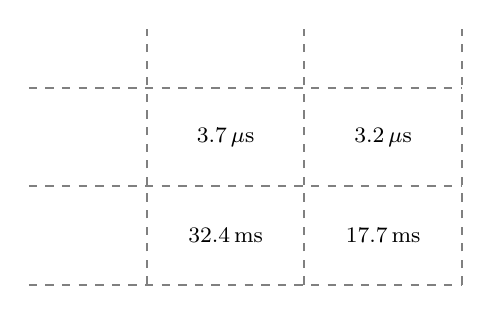
\begin{tikzpicture}
    \draw[dashed, thick, gray] (0.5,0) grid[xstep=2, ystep=1.25] (6,3.25);

    \node[anchor=east] at (1.75, 1.875) {\tool{}};
    \node[anchor=east] at (1.75, 0.625) {\toolL{}};

    \node[anchor=south] at (3, 2.65) {\tAH{}};
    \node[anchor=south] at (5, 2.75) {\tRH{}};

    \node at (3, 1.875) {\footnotesize $3.7\,\mu$s}; % any hit WH
    \node at (5, 1.875) {\footnotesize $3.2\,\mu$s}; % row hit WH

    \node at (3, 0.625) {\footnotesize $32.4\,$ms}; % any hit L
    \node at (5, 0.625) {\footnotesize $17.7\,$ms}; % any hit L
\end{tikzpicture}

    \end{minipage}
\end{frame}

\begin{frame}
    \frametitle{\tool{} Evaluation - \tAH{}}
    \input{figs/rtas22b/comp-eval-ah.tex}
\end{frame}

\begin{frame}
    \frametitle{\tool{} Evaluation - \tRH{}}
    \input{figs/rtas22b/comp-eval-rh.tex}
\end{frame}

